% !TeX spellcheck = en_US
% !TeX encoding = UTF-8

% COMPILE WITH:
% `latexmk`
% You need lualatex and biber (in all TeXLive distributions)

\documentclass[
numbers=noenddot,
fontsize=11pt,
paper=a4,
oneside,
titlepage,
bibliography=totoc,
chapterprefix=false,
DIV=calc,
headheight=14pt,
footheight=14pt,
%    draft
]{scrbook}

% LuaLaTeX-compatible font, graphics, spacing, and typography support.
\usepackage{fontspec}
\usepackage{graphicx}
\usepackage{geometry}
\geometry{a4paper,margin=2cm,includeheadfoot}
\usepackage{setspace}
\setstretch{1}
\usepackage[protrusion=false]{microtype}
\usepackage{etoolbox}
\usepackage{needspace}

% better language support
\usepackage{polyglossia}
\setdefaultlanguage{english}
\setotherlanguage{german}

\usepackage{tocbasic}
\usepackage{booktabs}
\usepackage{tikz}
\usetikzlibrary{positioning,arrows.meta}
\usepackage{tabularx}
\usepackage{multicol}
\usepackage{multirow}

\usepackage{scrlayer-scrpage}

% better bibliography (biblatex style)
% use biber to compile
\usepackage[citestyle=alphabetic, bibstyle=alphabetic, sorting=nyt, backend=biber, language=english, backref=true, maxcitenames=2]{biblatex}
% better quotes
% use \enquote{text}
\usepackage[autostyle,english=american,german=quotes]{csquotes}
\addbibresource{bibliography.bib}

% appendix
\usepackage[titletoc]{appendix}

% Allow natural line breaking in long prose, code fragments, and URLs.
\setlength{\emergencystretch}{6em}
% Keep the bibliography compact enough for the report page limit.
\AtBeginBibliography{\footnotesize\sloppy\raggedright}
\setlength{\bibitemsep}{0pt}
\setlength{\bibnamesep}{0pt}
\setlength{\bibinitsep}{0pt}
% Omit titles only for redundant online/news sources while retaining authors,
% dates, URLs, and citation information.
\AtEveryBibitem{\ifkeyword{notitle}{\clearfield{title}}{}}
\setcounter{biburlnumpenalty}{0}
\setcounter{biburlucpenalty}{0}
\setcounter{biburllcpenalty}{0}

% Compact, continuous sectioning for the requested short A4 layout.
\newcommand*{\compactchapterspace}{\par}
\AddtoDoHook{heading/preinit/chapter}{\compactchapterspace}
\RedeclareSectionCommand[beforeskip=0pt,afterskip=0.45\baselineskip]{chapter}
\RedeclareSectionCommand[beforeskip=0.75\baselineskip,afterskip=0.2\baselineskip]{section}
\RedeclareSectionCommand[beforeskip=0.5\baselineskip,afterskip=0.15\baselineskip]{subsection}
\RedeclareSectionCommand[beforeskip=0.4\baselineskip]{paragraph}
\setkomafont{chapter}{\normalfont\Large\bfseries}
\setkomafont{section}{\normalfont\large\bfseries}
\setkomafont{subsection}{\normalfont\normalsize\bfseries}
\setlength{\parindent}{0pt}
\setlength{\parskip}{0.5pt plus 0.25pt minus 0.25pt}
\setlength{\textfloatsep}{5pt plus 2pt minus 2pt}
\setlength{\floatsep}{4pt plus 2pt minus 2pt}
\setlength{\intextsep}{5pt plus 2pt minus 2pt}
\setlength{\abovecaptionskip}{2pt}
\setlength{\belowcaptionskip}{0pt}
\setcounter{topnumber}{5}
\setcounter{bottomnumber}{5}
\setcounter{totalnumber}{10}
\renewcommand{\topfraction}{0.95}
\renewcommand{\bottomfraction}{0.95}
\renewcommand{\textfraction}{0.05}
\renewcommand{\floatpagefraction}{0.8}

% where to put all images and figures
\graphicspath{{images/}{../SS/}{../outputs/task3/figures/}{../outputs/task4/figures/}}

% YOUR PACKAGES
\usepackage{xcolor}
\usepackage{placeins}
\usepackage{listings}
\usepackage{subcaption}
\setmonofont{DejaVu Sans Mono}[Scale=MatchLowercase]

% Python listing style (code is included from the real source files)
\lstdefinestyle{py}{
	language=Python,
	basicstyle=\ttfamily\scriptsize,
	numbers=left,
	numberstyle=\tiny\color{gray},
	frame=tb,
	breaklines=true,
	columns=fullflexible,
	showstringspaces=false,
	keepspaces=true,
	extendedchars=true,
	keywordstyle=\color{blue!60!black},
	commentstyle=\color{green!40!black}\itshape,
	stringstyle=\color{red!50!black},
	aboveskip=4pt,
	belowskip=2pt,
	captionpos=t,
	literate=
		{→}{{\texttt{->}}}1
		{−}{{-}}1
		{≥}{{>=}}1
		{≤}{{<=}}1
		{×}{{x}}1
		{�}{{?}}1
}
\lstset{style=py}
\renewcommand{\lstlistingname}{Listing}

% Screenshot figure: shows the image if ../SS/<name>.png exists, else a pending box
\newcommand{\ssfig}[4][\linewidth]{%
	\begin{figure}[htb]
		\centering
		\IfFileExists{../SS/#2.png}{\includegraphics[width=#1]{../SS/#2.png}}{\fbox{\parbox{0.8\linewidth}{\centering\vspace{0.5cm}Screenshot #2 pending\vspace{0.5cm}}}}
		\caption{#3}\label{#4}
	\end{figure}}


% Title
\title{Lab 2: Machine Learning for Network Attack Detection\\[0.4em]\Large CIC-IDS2017 Friday DDoS Dataset}

% Author
\newcommand{\authorA}{Justlyn Kaniyanthara Johnson}
\newcommand{\authorB}{Aayush Kapoor}
\author{\authorA \& \authorB}

% Group and matriculation numbers (used on the title page)
\newcommand{\groupno}{8}
\newcommand{\matrA}{121024}
\newcommand{\matrB}{120957}

% Date
\date{\today}

% CHOOSE ACCORDINGLY
%\newcommand{\thesisType}{Bachelorarbeit}
\newcommand{\thesisType}{MasterLab}

\makeatletter
\let\thetitle\@title
\let\theauthor\@author
\let\thedate\@date
\patchcmd{\scr@startchapter}
{\if@openright\cleardoublepage\else\clearpage\fi}
{}{}
{\PackageError{compact-layout}{Continuous chapter patch failed}
	{Check the installed KOMA-Script chapter implementation.}}
\makeatother

% PDF metadata and robust links. Keep this near the end of the preamble.
\usepackage{hyperref}
\hypersetup{
	unicode=true,
	hidelinks,
	pdftitle={Lab 2: Machine Learning for Network Attack Detection (CIC-IDS2017 Friday DDoS)},
	pdfauthor={\theauthor}
}

\pagestyle{scrheadings}
\automark[chapter]{chapter}
\chead{\leftmark}

\begin{document}
	
	%%%%%%%%%%%%%%%%%%%%%%%%%%%%%%%%%%%%%%%%%%%%%%%%%%%%%%%%%%%%%%%%%%%%%%%%%%%%%%%%%%%%%%%%%
	\frontmatter
	% CHOOSE ACCORDINGLY
	%% !TeX spellcheck = en_US
% !TeX encoding = UTF-8
\begin{titlepage}
    \centering
    \begin{onehalfspace}
    	\begin{german}
        	
\includegraphics[width=7cm]{uni-logo.png}\\
        	\vspace{1.0cm}
        	\large {\bfseries Lehrstuhl für Informatik mit Schwerpunkt\\ \textenglish{Digital Libraries and Web Information Systems}} \\

        	\vspace{2.5cm}

            \begin{doublespace}
            	\textenglish{\textsf{\Huge{\thetitle}}}
            \end{doublespace}

        	\vspace{2cm}

            \Large{Bachelorarbeit von}\\

        	\vspace{1cm}

        	{\bfseries \large{\theauthor}}

        	\vfill

        	{\large
        		\begin{tabular}[l]{cc}
        			\textsc{Prüfer}\\
        			Prof.~Dr.~Siegfried Handschuh
        		\end{tabular}
        	}

        	\vspace{1.5cm}

        	\parbox{\linewidth}{\hrule\strut}

            \vfill

	    \textgerman{\thedate}
    	\end{german}
    \end{onehalfspace}
\end{titlepage}

	% !TeX spellcheck = en_US
% !TeX encoding = UTF-8
\begin{titlepage}
    \centering
    \begin{onehalfspace}
    	\begin{german}
        	
\includegraphics[width=7cm]{uni-logo.png}\\
        	\vspace{1.0cm}
        	\large {\bfseries Security Insider Lab I}\\ 

        	\vspace{2.5cm}

            \begin{doublespace}
            	\textenglish{\textsf{\Huge{\thetitle}}}
            \end{doublespace}

        	\vspace{2cm}

			{\large Group \groupno}

        	\vspace{1cm}

        	\vfill

        	{\large
        		\begin{tabular}[l]{ll}
        			\authorA & \matrA \\
        			\authorB & \matrB \\
        			
        		\end{tabular}
        	}

        	\vspace{1.5cm}

        	\parbox{\linewidth}{\hrule\strut}

            \vfill

	    \textgerman{\thedate}
    	\end{german}
    \end{onehalfspace}
\end{titlepage}

	
	\tableofcontents
	
	% -- ABSTRACT
	\clearpage
	% !TeX spellcheck = en_US
% !TeX encoding = UTF-8
\chapter*{Abstract}

In the second lab of the Security Insider Lab, we detect network attacks from flow features with machine learning. We first recorded our own traffic and converted it into flows with CICFlowMeter. Our first captures were mostly IPv6 and produced bogus flows, because CICFlowMeter force-parses non-IPv4 frames as IPv4. With IPv6 disabled, we obtained 569 flows, 547 of them valid TCP/UDP flows. As training data we use the Friday-afternoon DDoS file of CIC-IDS2017, which has 225,745 flows, 128,027 of them DDoS. Pre-processing removed infinite values, duplicate rows and constant and identical columns, which left 223,082 flows with 59 features. We then made a stratified split, min-max scaled the features and selected the 20 best with $\chi^2$. We trained Logistic Regression and Decision Tree classifiers for the binary target BENIGN vs.\ DDoS. The default Decision Tree is best: on the test split of 66,925 flows it makes 7 false positives and 25 false negatives (DDoS F1 0.9996), whereas Logistic Regression raises about 2,000 false alarms (DDoS F1 0.974). Class weighting changes almost nothing, because DDoS is the majority class. Applied flow by flow to our own benign capture, the Decision Tree classified all 547 valid flows as BENIGN, so it raised no false alarm. Since the capture contains no attack, we cannot measure the detection rate there, and the near-perfect benchmark scores may partly rest on shortcut features such as the destination port.

	
	% -- Acknowledgements (optional, left out)
	% % !TeX spellcheck = en_US
% !TeX encoding = UTF-8
\chapter*{Acknowledgments}

% I would first like to thank my thesis advisor ...
	% \newpage
	
	% -- List of figures
\vspace{4\baselineskip}
\listoffigures

% -- List of tables
\vspace{4\baselineskip}
\listoftables

% -- List of listings
\vspace{4\baselineskip}
\lstlistoflistings
	
	%%%%%%%%%%%%%%%%%%%%%%%%%%%%%%%%%%%%%%%%%%%%%%%%%%%%%%%%%%%%%%%%%%%%%%%%%%%%%%%%%%%%%%%%%
	\mainmatter
	
	% -- Chapters
	% following IMRaD structure
	% adjust for your liking
	% !TeX encoding = UTF-8
\chapter{Introduction}\label{chap:introduction}

In the second lab of the Security Insider Lab, we detect network attacks with machine learning. Instead of inspecting packets one by one, we describe each network connection by a vector of statistical features (a \emph{flow}) and train classifiers to tell benign flows from attack flows. The lab has four tasks:

\begin{enumerate}\setlength\itemsep{0pt}
	\item \textbf{Task 1:} we capture our own traffic and convert it into flows with CICFlowMeter.
	\item \textbf{Task 2:} we analyze a labeled flow dataset, CIC-IDS2017.
	\item \textbf{Task 3:} we pre-process the dataset: we handle infinite and missing values, scale the features, and select the 20 most informative ones.
	\item \textbf{Task 4:} we train Logistic Regression and Decision Tree classifiers, evaluate them, and apply the best model to the flows of our own capture.
\end{enumerate}

\paragraph{Dataset.} As suggested in the lab slides, we use the Friday-afternoon DDoS file of CIC-IDS2017, \texttt{Friday-WorkingHours-Afternoon-DDos.csv}. It contains benign flows and flows of a distributed denial-of-service attack, so the task is a binary classification problem, BENIGN vs.\ DDoS.

\paragraph{Structure.} Chapter~\ref{chap:task1_flows} describes how we produced flows from our own capture and the problems we ran into. Chapter~\ref{chap:task2_dataset} introduces the dataset, Chapter~\ref{chap:task3_preprocessing} the pre-processing, and Chapter~\ref{chap:task4_ml} the classifiers and their evaluation. Chapter~\ref{chap:task4_realtime} applies the best model to our own flows, and Chapter~\ref{chap:discussion} discusses the results and limitations. All code is in our \texttt{ddosids} Python package; the listings in this report are excerpts of the real source files.

	% !TeX encoding = UTF-8
\chapter{Task 1: Network Flows with CICFlowMeter}\label{chap:task1_flows}

\section{What a Flow Is}\label{sec:flow}

A flow summarizes a bidirectional exchange of packets between two endpoints, identified by source and destination IP address, ports and protocol. CICFlowMeter~\cite{lashkari2017cicflowmeter,cicflowmeter_github} reads a packet capture and writes one row per flow with 84 columns: identifying metadata (flow ID, addresses, ports, protocol, timestamp), 77 numeric features (packet counts and lengths, inter-arrival times, TCP flag counts, window sizes, idle and active times) and a label column. A flow ends when a FIN or RST is seen, or when a timeout expires: 5\,s without activity (activity timeout) or 120\,s of total flow duration (flow timeout). CICFlowMeter only writes flows with at least two packets, so single-packet exchanges, such as a lone DNS query or a traceroute probe, do not appear in the output.

\section{Capture Setup}\label{sec:capture}

We recorded our own traffic with Wireshark while browsing, resolving names and running the Steam client. The final capture, \texttt{task1\_lab2.pcapng}, has 81,110 frames over 347.4\,s (2026-11-04, 16:05--16:10). We converted it offline with CICFlowMeter to \texttt{task2\_lab2.pcap\_Flow.csv}. This file is the real-time input of Chapter~\ref{chap:task4_realtime}. Since the traffic is ordinary browsing, we treat all flows as benign by construction.

\ssfig[0.65\linewidth]{SS25}{CICFlowMeter in offline mode converting the capture, under its original file name \texttt{benign\_lab2\_3.pcap}, with the default timeouts (120\,s flow, 5\,s activity): 81,110 packets read (81,109 valid, 1 discarded), the same packet count as \texttt{task1\_lab2.pcapng}. The reported \enquote{Total 570 flows} counts the lines of the output CSV including its header, i.e.\ 569 flows.}{fig:ss25}

\section{The IPv6 Problem}\label{sec:ipv6}

Our first two captures produced CSV files in which most flows were garbage: protocol 0, port 0 and implausible IP addresses. Table~\ref{tab:captures} compares the captures. In the first two, 89--98\,\% of the frames were IPv6. After we disabled IPv6 on the capturing laptop for the third capture with \texttt{sudo sysctl -w net.ipv6.conf.all.disable\_ipv6=1} (Figure~\ref{fig:ss24}), only 24 IPv6 frames (0.03\,\%) remained and the share of valid flows rose from 15\,\% and 5\,\% to 96\,\%.

\ssfig[0.55\linewidth]{SS24}{Disabling IPv6 on the capturing laptop before the third capture; \texttt{sysctl} confirms \texttt{net.ipv6.conf.all.disable\_ipv6 = 1}.}{fig:ss24}

\begin{table}[ht]
	\centering\small
	\begin{tabular}{lrrrrrr}
		\toprule
		Capture & Frames & IPv6 frames & Flows & Protocol 0 & Valid TCP/UDP \\
		\midrule
		1st (since deleted) & 129,548 & 126,904 (98\,\%) & 532 & 454 & 78 \\
		2nd (since deleted) & 98,780 & 88,458 (89.5\,\%) & 1,327 & 1,260 & 67 \\
		3rd, IPv6 off (final) & 81,110 & 24 (0.03\,\%) & 569 & 22 & 547 \\
		\bottomrule
	\end{tabular}
	\caption{The three captures. Only the third, with IPv6 disabled, yields mostly valid flows.}
	\label{tab:captures}
\end{table}

\paragraph{Root cause.} We traced the problem in the CICFlowMeter source. IPv6 support is switched off in the code: \texttt{readIP6 = false} is hard-coded in \texttt{Cmd.java} (line 126) and \texttt{ReadPcapFileWorker.java} (line 152). Every frame that is not IPv4 (IPv6, ARP, HomePlug powerline frames) falls through to \texttt{getVPNInfo()}, which force-parses the raw frame as an IPv4 header starting at byte 0. The fake ``source IP'' is therefore just the EtherType plus two further bytes, and the fake ``destination IP'' is taken from the IPv6 flow label and payload length (Table~\ref{tab:fakeip}). The IPv4 flows themselves are parsed correctly. We decided against enabling CICFlowMeter's IPv6 path, because its UDP branch wrongly reads the header length from the TCP header (\texttt{PacketReader.java}, line 204). With IPv6 off, our flows are IPv4-only, like the training data.

\begin{table}[ht]
	\centering\small
	\begin{tabular}{llp{7.5cm}}
		\toprule
		Fake ``IP'' & Bytes & Actually \\
		\midrule
		\texttt{134.221.96.0} & \texttt{86 DD 60 00} & EtherType 0x86DD (IPv6) and first IPv6 header bytes \\
		\texttt{0.0.4.214} (dst) & \texttt{00 00 04 D6} & IPv6 flow label and payload length (1238) \\
		\texttt{136.225.0.0} & \texttt{88 E1 \ldots} & EtherType 0x88E1 (HomePlug AV) \\
		\texttt{8.6.x.x} & \texttt{08 06 \ldots} & EtherType 0x0806 (ARP) \\
		\bottomrule
	\end{tabular}
	\caption{How non-IPv4 frames turn into fake IP addresses in the CICFlowMeter output.}
	\label{tab:fakeip}
\end{table}

\section{The Final Capture}\label{sec:final-capture}

\ssfig[0.8\linewidth]{SS15}{Protocol hierarchy of \texttt{task1\_lab2.pcapng} in Wireshark: 99.94\,\% of the frames are IPv4, only 24 are IPv6.}{fig:ss15}
\ssfig[0.8\linewidth]{SS17}{First rows of \texttt{task2\_lab2.pcap\_Flow.csv} in LibreOffice Calc: flow ID, endpoints, protocol, timestamp and the first features. (The \texttt{Label} column further to the right reads \texttt{NeedManualLabel}.)}{fig:ss17}

The final capture contains 47,682 UDP frames (29,682 QUIC, 580 DNS), 33,218 TCP frames (11,994 TLS, 26 HTTP), 160 ICMP frames and 26 ARP frames (Figure~\ref{fig:ss15}). Its offline conversion (Figure~\ref{fig:ss25}) yields 569 flows (Table~\ref{tab:t1flows}, Figure~\ref{fig:ss17}). More than half of the classified flows (289) are DNS queries to the local resolver, since every query is its own flow; 213 go to port 443 and 15 to port 80. The classified flows contain 80,705 packets, which is 99.8\,\% of the 80,900 IPv4 TCP/UDP frames. The missing packets are single-packet UDP exchanges, mostly traceroute probes, which CICFlowMeter does not write.

\begin{table}[ht]
	\centering\small
	% AUTO-GENERATED by scripts/make_report_tables.py from task2_lab2.pcap_Flow.csv -- do not edit
\begin{tabular}{lr}
\toprule
Quantity & Value \\
\midrule
Total flows & 569 \\
TCP flows (6) & 162 \\
UDP flows (17) & 385 \\
Protocol 0 flows (dropped) & 22 \\
Flows classified (TCP + UDP) & 547 \\
Packets in classified flows & 80\,705 \\
Top-1 destination port & 53 (289 flows) \\
Top-2 destination port & 443 (213 flows) \\
Top-3 destination port & 80 (15 flows) \\
\bottomrule
\end{tabular}

	\caption{Flows of \texttt{task2\_lab2.pcap\_Flow.csv}. The 22 flows with protocol 0 are not TCP/UDP flows and are dropped before classification.}
	\label{tab:t1flows}
\end{table}

The 22 protocol-0 flows consist of 15 real ICMP flows (CICFlowMeter only sets the protocol number for TCP and UDP), 4 flows from left-over IPv6 frames and 3 from ARP frames, the last two groups mis-parsed as described above. The real-time detector drops all 22 (3.9\,\%) and logs the count. There are no infinite or NaN values in the remaining flows, and all 77 features map to the training feature names (Section~\ref{sec:realtime-setup}). About 70\,\% of the valid flows are UDP (DNS, QUIC and Steam). The application mix (e.g.\ QUIC and Steam) and the network itself differ from the 2017 testbed, so we expect domain shift (Chapter~\ref{chap:task4_realtime}).


\FloatBarrier

	% !TeX encoding = UTF-8
\chapter{Task 2: The CIC-IDS2017 Dataset}\label{chap:task2_dataset}

CIC-IDS2017 was created by the Canadian Institute for Cybersecurity at the University of New Brunswick~\cite{sharafaldin2018cicids,cicids2017_web}. The flows were extracted with CICFlowMeter~\cite{lashkari2017cicflowmeter}. We use the pre-computed ``MachineLearningCSV'' file \texttt{Friday-WorkingHours-Afternoon-DDos.csv} (77\,MB). It has 225,745 flows and 79 columns: 78 numeric flow features and the \texttt{Label}. It contains no flow ID, IP address or timestamp columns, but \texttt{Destination Port} is present. The file covers the DDoS attack of the Friday afternoon, as described in the dataset paper.

The file has two labels, BENIGN and DDoS, and the attack is the \emph{majority} class: DDoS makes up 56.71\,\% of the raw flows (Table~\ref{tab:t2labels}). The classes are therefore reasonably balanced, and accuracy is less misleading than on a dataset with a rare attack. We still report per-class precision, recall and F1, the macro-F1 and confusion matrices throughout, never accuracy alone. Virtually all DDoS flows target destination port 80, while benign traffic is spread over several ports (mostly 53, 443 and 80). Models can exploit this as a shortcut (Section~\ref{sec:t3-interp} and Chapter~\ref{chap:discussion}).

\begin{table}[ht]
	\centering\small
	% AUTO-GENERATED by scripts/make_report_tables.py from outputs/task3/label_summary_{raw,clean}.csv -- do not edit
\begin{tabular}{lrrrr}
\toprule
Label & Raw & Share & Cleaned & Share \\
\midrule
BENIGN & 97\,718 & 43.29\,\% & 95\,068 & 42.62\,\% \\
DDoS & 128\,027 & 56.71\,\% & 128\,014 & 57.38\,\% \\
\midrule
\textbf{Total} & \textbf{225\,745} & \textbf{100.00\,\%} & \textbf{223\,082} & \textbf{100.00\,\%} \\
\bottomrule
\end{tabular}

	\caption{Label distribution of the Friday file, raw and after the cleaning steps of Chapter~\ref{chap:task3_preprocessing}.}
	\label{tab:t2labels}
\end{table}


\FloatBarrier

	% !TeX encoding = UTF-8
\chapter{Task 3: Data Pre-processing}\label{chap:task3_preprocessing}

The task asks us to analyze the labels, handle infinite and NaN values, scale the features with min-max scaling and select the 20 best features with \texttt{SelectKBest}. We implemented this in Python 3.12 with pandas and scikit-learn~\cite{pedregosa2011sklearn} (modules \texttt{data.py} and \texttt{features.py}, script \texttt{task3\_preprocess.py}). The steps are, in this order:

\begin{enumerate}\setlength\itemsep{0pt}
	\item \textbf{Load and analyze labels.} 65 of the 79 column names carry stray leading spaces and are stripped. The labels are normalized (whitespace collapsed, validated against the two expected classes). For this file this step changes nothing, because the labels are already clean.
	\item \textbf{Drop the duplicate column.} \texttt{Fwd Header Length} appears twice in the header, a known artifact of the CICFlowMeter export. We drop the second copy.
	\item \textbf{Infinity and NaN.} We replace $\pm\infty$ by NaN and \emph{drop} the affected rows. Only 34 rows are affected, 32 BENIGN and 2 DDoS, so dropping loses almost no information and introduces no artificial values. The infinite and NaN values occur only in \texttt{Flow Bytes/s} and \texttt{Flow Packets/s}: CICFlowMeter divides by the flow duration, which is 0 for some flows (a positive byte count divided by 0 gives $\infty$, 0/0 gives NaN).
	\item \textbf{Duplicate rows.} We remove exact duplicates before splitting. Otherwise identical rows land in both train and test sets and inflate the test scores.
	\item \textbf{Constant columns.} They carry no information and trigger warnings in \texttt{SelectKBest}.
	\item \textbf{Identical columns.} Columns equal to an earlier one (tolerance $10^{-6}$) are removed, so that the 20 selected features are distinct. The tolerance is needed for one pair, \texttt{Bwd Packet Length Mean} and \texttt{Avg Bwd Segment Size}: they are the same quantity but differ in 2 rows by at most $10^{-6}$ because of CSV rounding.
	\item \textbf{Train/test split.} A stratified 70/30 split on the label with \texttt{random\_state=42}, done \emph{before} anything is fitted.
	\item \textbf{Min-max scaling.} \texttt{MinMaxScaler(clip=True)} maps each feature to $[0,1]$. It is fitted on the training set only, so no test statistics leak into training, and \texttt{clip=True} keeps unseen values, such as live traffic later, inside $[0,1]$.
	\item \textbf{Feature selection.} \texttt{SelectKBest(chi2, k=20)} on the scaled training set. We scale first because $\chi^2$ requires non-negative input, and the raw data contains negative values: \texttt{Init\_Win\_bytes\_*} is $-1$ when no window was observed, and a few durations are negative.
\end{enumerate}

The column-level steps 5 and 6 use feature values only, never labels, so they leak no label information. Listing~\ref{lst:clean} shows the core of steps 2--6 in the code.

% U+FFFD in data.py (normalize_labels) would otherwise leak into the listing (listings/LuaTeX quirk)
{\catcode"FFFD=9 \lstinputlisting[style=py,float=htbp,linerange={113-114,118-121,134-136,141-143,148-150,155-157},caption={Core cleaning steps of \texttt{clean()} in \texttt{src/ddosids/data.py} (steps 2--6; logging calls omitted)},label={lst:clean}]{../src/ddosids/data.py}}

\section{Results}\label{sec:t3-results}

\ssfig[0.45\linewidth]{SS27}{Raw label summary as printed by the pre-processing script: 97,718 BENIGN and 128,027 DDoS flows (cf.\ Table~\ref{tab:t2labels}).}{fig:ss27}

Table~\ref{tab:t3cleaning} lists the cleaning steps with their effect (Figure~\ref{fig:ss28} shows the script log), and Table~\ref{tab:t3removed} the removed columns. The raw file has 2,633 duplicate rows, but 4 of them contain infinite or NaN values and are already gone after step 3, so step 4 drops 2,629 (2,618 BENIGN, 11 DDoS). The six bulk-transfer features are always 0 in this CICFlowMeter version. \texttt{Fwd PSH Flags} is identical to \texttt{SYN Flag Count}, although PSH and SYN are different TCP flags. This points to a feature-extraction problem in the CICFlowMeter version used for CIC-IDS2017, in line with the literature~\cite{engelen2021troubleshooting}.

\begin{table}[ht]
	\centering\small
	% AUTO-GENERATED by scripts/make_report_tables.py from outputs/task3/cleaning_report.json -- do not edit
\begin{tabularx}{\linewidth}{rlrrX}
\toprule
\# & Step & Rows & Cols & Detail \\
\midrule
1 & Drop duplicate header column & 225\,745$\to$225\,745 & 79$\to$78 & $-$1 column (\texttt{Fwd Header Length.1}) \\
2 & Replace $\pm\infty$ by NaN & 225\,745$\to$225\,745 & 78$\to$78 & inf: \texttt{Flow Bytes/s} 30, \texttt{Flow Packets/s} 34; NaN: \texttt{Flow Bytes/s} 4 \\
3 & Drop NaN rows & 225\,745$\to$225\,711 & 78$\to$78 & $-$34 rows (32 BENIGN, 2 DDoS) \\
4 & Drop duplicate rows & 225\,711$\to$223\,082 & 78$\to$78 & $-$2\,629 rows (2\,618 BENIGN, 11 DDoS) \\
5 & Drop constant columns & 223\,082$\to$223\,082 & 78$\to$68 & $-$10 columns \\
6 & Drop identical columns & 223\,082$\to$223\,082 & 68$\to$60 & $-$8 columns \\
\midrule
 & \textbf{Result} & \textbf{223\,082} &  & \textbf{223\,082 rows $\times$ 59 features} \\
\bottomrule
\end{tabularx}

	\caption{Cleaning steps. The column counts include the \texttt{Label} column, so the 60 remaining columns are 59 features plus \texttt{Label}. Loading and label normalization happen before step 1.}
	\label{tab:t3cleaning}
\end{table}

\ssfig{SS28}{Cleaning steps as logged by the pre-processing script, ending with \enquote{Final: 223082 rows x 59 features} (cf.\ Table~\ref{tab:t3cleaning}).}{fig:ss28}

\begin{table}[ht]
	\centering\small
	% AUTO-GENERATED by scripts/make_report_tables.py from outputs/task3/cleaning_report.json -- do not edit
\begin{tabularx}{\linewidth}{lX}
\toprule
Kind & Columns \\
\midrule
Constant (10) & \texttt{Bwd PSH Flags}, \texttt{Fwd URG Flags}, \texttt{Bwd URG Flags}, \texttt{CWE Flag Count}, \texttt{Fwd Avg Bytes/Bulk}, \texttt{Fwd Avg Packets/Bulk}, \texttt{Fwd Avg Bulk Rate}, \texttt{Bwd Avg Bytes/Bulk}, \texttt{Bwd Avg Packets/Bulk}, \texttt{Bwd Avg Bulk Rate} \\
\midrule
Identical & \texttt{Fwd PSH Flags} $\to$ \texttt{SYN Flag Count} (dropped) \\
Identical & \texttt{RST Flag Count} $\to$ \texttt{ECE Flag Count} (dropped) \\
Identical & \texttt{Fwd Packet Length Mean} $\to$ \texttt{Avg Fwd Segment Size} (dropped) \\
Identical & \texttt{Bwd Packet Length Mean} $\to$ \texttt{Avg Bwd Segment Size} (dropped) \\
Identical & \texttt{Total Fwd Packets} $\to$ \texttt{Subflow Fwd Packets} (dropped) \\
Identical & \texttt{Total Length of Fwd Packets} $\to$ \texttt{Subflow Fwd Bytes} (dropped) \\
Identical & \texttt{Total Backward Packets} $\to$ \texttt{Subflow Bwd Packets} (dropped) \\
Identical & \texttt{Total Length of Bwd Packets} $\to$ \texttt{Subflow Bwd Bytes} (dropped) \\
\bottomrule
\end{tabularx}

	\caption{Removed columns. For identical pairs, the first column is kept and the second one dropped.}
	\label{tab:t3removed}
\end{table}

After cleaning, 223,082 flows with 59 features remain: 95,068 BENIGN and 128,014 DDoS (Table~\ref{tab:t2labels}), so DDoS stays the majority class. Table~\ref{tab:t3split} shows the split: the test set contains 66,925 flows, of which 38,404 are DDoS.

\begin{table}[ht]
	\centering\small
	% AUTO-GENERATED by scripts/make_report_tables.py from artifacts/clean.parquet, artifacts/split_indices.json -- do not edit
\begin{tabular}{lrr}
\toprule
Label & Train (70\,\%) & Test (30\,\%) \\
\midrule
BENIGN & 66\,547 & 28\,521 \\
DDoS & 89\,610 & 38\,404 \\
\midrule
\textbf{Total} & \textbf{156\,157} & \textbf{66\,925} \\
\bottomrule
\end{tabular}

	\caption{Stratified 70/30 split (\texttt{random\_state=42}).}
	\label{tab:t3split}
\end{table}

\ssfig[0.5\linewidth]{SS29}{Final label summary after cleaning and the class counts of the stratified 70/30 split (cf.\ Tables~\ref{tab:t2labels} and~\ref{tab:t3split}).}{fig:ss29}

On the training set, each of the six example features in Table~\ref{tab:t3scaling} has a scaled minimum of 0 and a maximum of 1. The durations and inter-arrival times, with maxima near the 120\,s timeout, are heavy-tailed and keep modest means after scaling.

\begin{table}[ht]
	\centering\small
	% AUTO-GENERATED by scripts/make_report_tables.py from outputs/task3/describe_train_{before,after}_scaling.csv -- do not edit
\begin{tabular}{lrrrrrr}
\toprule
 & \multicolumn{3}{c}{Before scaling} & \multicolumn{3}{c}{After scaling} \\
\cmidrule(lr){2-4}\cmidrule(lr){5-7}
Feature & Min & Max & Mean & Min & Max & Mean \\
\midrule
\texttt{Init\_Win\_bytes\_backward} & $-$1 & 65\,535 & 616.5311 & 0 & 1 & 0.0094 \\
\texttt{Init\_Win\_bytes\_forward} & $-$1 & 65\,535 & 4\,289 & 0 & 1 & 0.0655 \\
\texttt{Destination Port} & 0 & 65\,532 & 9\,036 & 0 & 1 & 0.1379 \\
\texttt{Flow Duration} & $-$1 & 119\,999\,937 & 16\,472\,365 & 0 & 1 & 0.1373 \\
\texttt{Bwd IAT Total} & 0 & 120\,000\,000 & 6\,626\,749 & 0 & 1 & 0.0552 \\
\texttt{PSH Flag Count} & 0 & 1 & 0.3556 & 0 & 1 & 0.3556 \\
\bottomrule
\end{tabular}

	\caption{Six example features of the training set before and after min-max scaling.}
	\label{tab:t3scaling}
\end{table}

\texttt{URG Flag Count} and \texttt{Destination Port} lead the 20 selected features (Table~\ref{tab:t3top20}; scores in Figure~\ref{fig:fsbin}, script output in Figure~\ref{fig:ss30}) with scores above 28,000 each, and the scores fall steadily down the ranking.

\begin{table}[ht]
	\centering\small
	% AUTO-GENERATED by scripts/make_report_tables.py from outputs/task3/feature_scores_binary.csv -- do not edit
\begin{tabular}{rlr}
\toprule
Rank & Binary feature & $\chi^2$ \\
\midrule
1 & \texttt{URG Flag Count} & 30058.11 \\
2 & \texttt{Destination Port} & 28476.04 \\
3 & \texttt{Bwd Packet Length Max} & 22196.57 \\
4 & \texttt{Bwd Packet Length Std} & 15201.54 \\
5 & \texttt{Bwd Packet Length Mean} & 13631.13 \\
6 & \texttt{Bwd IAT Total} & 10104.71 \\
7 & \texttt{Max Packet Length} & 9940.91 \\
8 & \texttt{Packet Length Mean} & 9735.77 \\
9 & \texttt{Fwd Packet Length Max} & 9338.26 \\
10 & \texttt{Packet Length Std} & 9282.63 \\
11 & \texttt{Average Packet Size} & 8361.12 \\
12 & \texttt{Fwd Packet Length Mean} & 8326.59 \\
13 & \texttt{Fwd PSH Flags} & 7104.49 \\
14 & \texttt{Packet Length Variance} & 6816.96 \\
15 & \texttt{Bwd IAT Max} & 6626.18 \\
16 & \texttt{Fwd Packet Length Std} & 6519.34 \\
17 & \texttt{PSH Flag Count} & 5771.95 \\
18 & \texttt{Down/Up Ratio} & 4499.68 \\
19 & \texttt{Fwd Packet Length Min} & 3409.00 \\
20 & \texttt{Bwd IAT Std} & 3351.57 \\
\bottomrule
\end{tabular}

	\caption{The 20 best features by $\chi^2$ score (min-max-scaled training set), binary target.}
	\label{tab:t3top20}
\end{table}

\ssfig[0.5\linewidth]{SS30}{The top features by $\chi^2$ as printed by the pre-processing script (binary target, ranks 1--20; cf.\ Table~\ref{tab:t3top20}).}{fig:ss30}

\begin{figure}[ht]
	\centering
	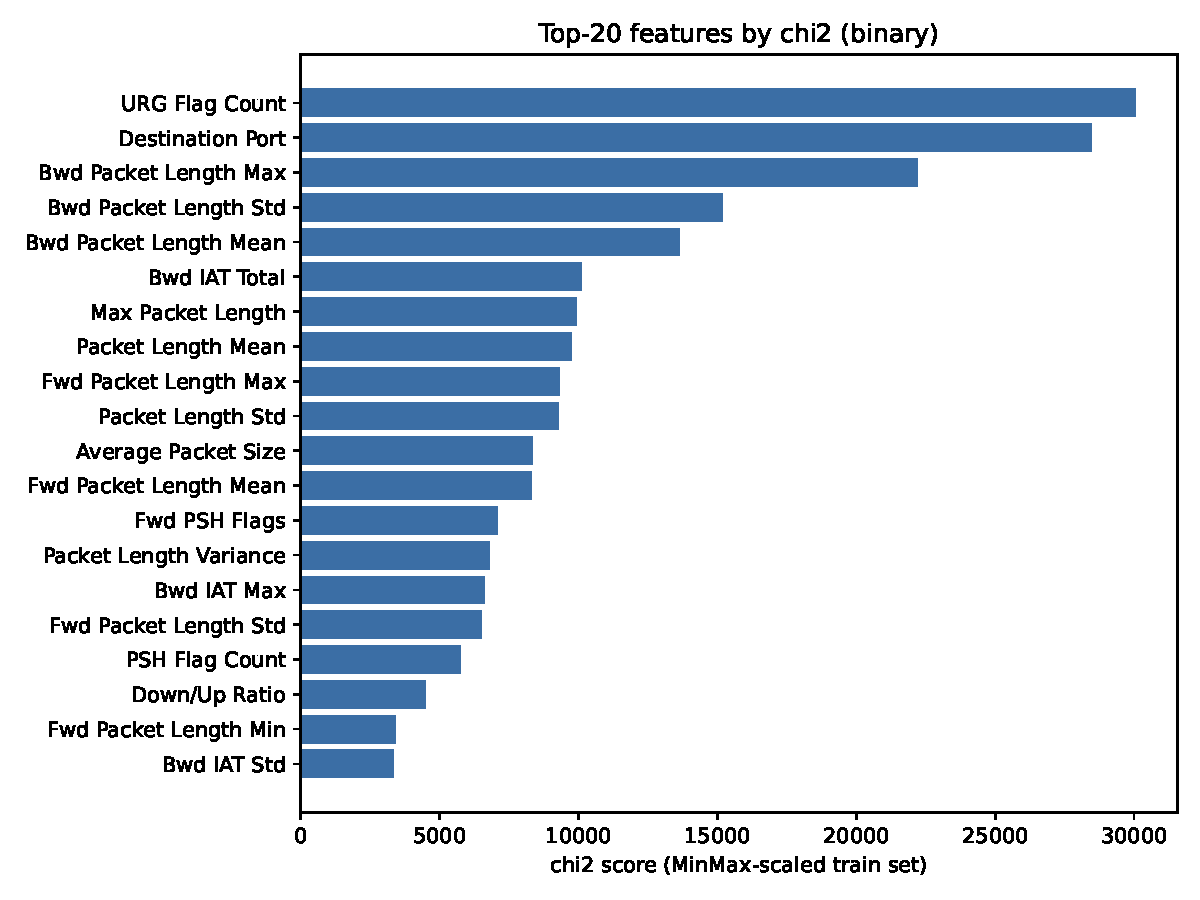
\includegraphics[width=0.75\linewidth]{feature_scores_binary.pdf}
	\caption{Top-20 flow features by $\chi^2$ score for binary classification (BENIGN vs.\ DDoS), computed on the min-max-scaled training set.}
	\label{fig:fsbin}
\end{figure}


\section{Interpretation}\label{sec:t3-interp}

The top-20 list is dominated by packet-size features: twelve of the 20 features describe packet lengths (forward and backward length statistics, the overall maximum, mean, standard deviation and variance, and the average packet size). This is plausible for a flooding attack, whose requests are likely more uniform than the mix of benign traffic. Three features are TCP flag counts (\texttt{URG Flag Count}, \texttt{Fwd PSH Flags}, \texttt{PSH Flag Count}), three describe backward inter-arrival times, and \texttt{Down/Up Ratio} captures the traffic asymmetry. \texttt{Destination Port} ranks second, and virtually all DDoS flows target port 80, so a model can learn ``port 80 is suspicious'' instead of the attack behavior. We expect such testbed-specific features to generalize poorly to other networks. The $\chi^2$ test on min-max-scaled continuous data is also only a heuristic: it treats scaled values like frequencies, and heavy-tailed features are squeezed towards 0, which lowers their scores. The ranking therefore depends on the scaling.

\FloatBarrier

	% !TeX encoding = UTF-8
\chapter{Task 4: Machine Learning Classifiers}\label{chap:task4_ml}

\section{Setup}\label{sec:ml-setup}

We train Logistic Regression (LR, \texttt{max\_iter=5000}) and a Decision Tree (DT, \texttt{random\_state=42}, unpruned) with scikit-learn~\cite{pedregosa2011sklearn}. Each is trained in two variants, default and \texttt{class\_weight="balanced"}. The file has only one attack class, so a multiclass target would duplicate the binary one (BENIGN vs.\ DDoS), and we train four binary models. Every model is one scikit-learn \texttt{Pipeline}: \texttt{MinMaxScaler(clip=True)}, \texttt{SelectKBest(chi2, k=20)} and the classifier (Listing~\ref{lst:pipe}). Scaler and selector are fitted on the training split only (156,157 flows). All models are evaluated on the held-out test split of 66,925 flows, of which 38,404 are DDoS. Inference time is the median of five timed \texttt{predict} calls on the whole test split after one warm-up call, scaled to 1,000 flows. Both LR models converged after 48 iterations, far below the limit of 5,000.

\lstinputlisting[style=py,float=htbp,linerange={22-27,30-38},caption={\texttt{build\_pipeline()} and \texttt{make\_classifier()} in \texttt{src/ddosids/models.py}},label={lst:pipe}]{../src/ddosids/models.py}

\section{Results}\label{sec:ml-binary}

The default DT makes only 7 false positives and 25 false negatives on 66,925 test flows (Table~\ref{tab:t4binary}), which gives a DDoS precision of 0.9998, a recall of 0.9993 and an F1 of 0.9996. Logistic Regression detects almost as many attacks (recall 0.9988, 45 missed flows) but raises about 2,000 false alarms (2,008 for the default and 1,974 for the balanced variant), so its DDoS precision is only about 0.95 and its F1 0.974. Figure~\ref{fig:cm} shows the confusion matrices of the default DT and the balanced LR, and Figure~\ref{fig:ss33} the console output for the default DT.

Class weighting changes almost nothing. For the DT, the balanced variant has exactly the same confusion matrix and metrics as the default one, and for LR the false positives drop only from 2,008 to 1,974. The two classes are close to balanced (57\,\% DDoS and 43\,\% BENIGN after cleaning), so \texttt{class\_weight="balanced"} gives both classes weights close to one. The fit and inference times come from a single run each.

\begin{table}[ht]
	\centering\small
	\resizebox{\linewidth}{!}{% AUTO-GENERATED by scripts/make_report_tables.py from outputs/task4/comparison.csv, outputs/task4/metrics.json -- do not edit
\begin{tabular}{lrrrrrrrrr}
\toprule
Model & Acc. & Macro-F1 & Prec. & Rec. & F1 & FP & FN & Fit (s) & Inf. (ms/1k) \\
\midrule
LR default & 0.9693 & 0.9683 & 0.9503 & 0.9988 & 0.9739 & 2\,008 & 45 & 6.45 & 0.717 \\
LR balanced & 0.9698 & 0.9689 & 0.9511 & 0.9988 & 0.9744 & 1\,974 & 45 & 5.97 & 1.996 \\
\textbf{DT default} & \textbf{0.9995} & \textbf{0.9995} & \textbf{0.9998} & \textbf{0.9993} & \textbf{0.9996} & \textbf{7} & \textbf{25} & \textbf{2.20} & \textbf{0.695} \\
DT balanced & 0.9995 & 0.9995 & 0.9998 & 0.9993 & 0.9996 & 7 & 25 & 1.25 & 0.717 \\
\bottomrule
\end{tabular}
}
	\caption{Binary results on the test split (Prec., Rec., F1 refer to the DDoS class; Macro-F1 averages both classes; FP/FN are false positives and false negatives). Best model in bold.}
	\label{tab:t4binary}
\end{table}

\begin{figure}[htb]
	\centering
	\begin{subfigure}[t]{0.48\linewidth}
		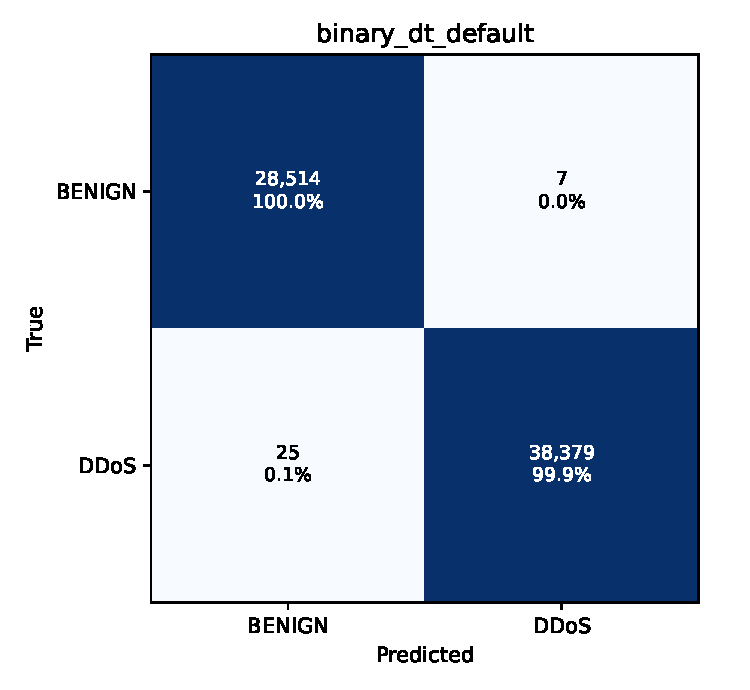
\includegraphics[width=\linewidth]{cm_binary_dt_default.pdf}
		\caption{Decision Tree (default): 7 false positives, 25 false negatives.}
	\end{subfigure}\hfill
	\begin{subfigure}[t]{0.48\linewidth}
		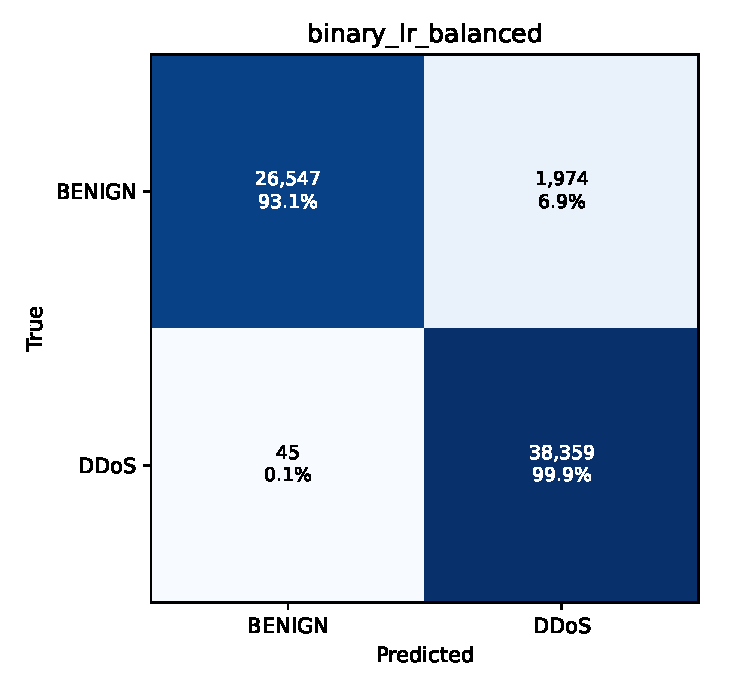
\includegraphics[width=\linewidth]{cm_binary_lr_balanced.pdf}
		\caption{Logistic Regression (balanced): 1,974 false positives, 45 false negatives.}
	\end{subfigure}
	\caption{Confusion matrices of two of the four models (test split).}
	\label{fig:cm}
\end{figure}

\ssfig[0.55\linewidth]{SS33}{Console output of the training script for the chosen model, \texttt{binary\_dt\_default}: per-class report, confusion matrix, and fit and inference times.}{fig:ss33}

\ssfig{SS35}{Comparison table of the four models, as printed by the training script (cf.\ Table~\ref{tab:t4binary}).}{fig:ss35}

\section{Interpretation}\label{sec:ml-interp}

The Decision Tree beats Logistic Regression in every metric of Table~\ref{tab:t4binary}: the DDoS F1 is 0.9996 against at most 0.9744. Attacks occupy narrow value ranges of a few features (packet lengths, port 80, flag counts), and a tree isolates such ranges with axis-aligned thresholds. LR draws a single linear boundary through heavy-tailed, min-max-compressed features and cannot separate the classes as sharply.

We use \texttt{binary\_dt\_default} in the real-time part. Default and balanced DT are identical on the test split, so we take the simpler default model, and it has the fewest errors of all four models. \texttt{Destination Port} is the second-best feature by $\chi^2$ (Table~\ref{tab:t3top20}), and virtually all DDoS flows target port 80, so the near-perfect scores may partly rest on the port as a shortcut (Chapter~\ref{chap:discussion}). Because the test split comes from the same capture as the training data, Chapter~\ref{chap:task4_realtime} also checks the model on traffic from a different network.

\FloatBarrier

	% !TeX encoding = UTF-8
\chapter{Task 4: Real-Time Classification}\label{chap:task4_realtime}

\section{Setup}\label{sec:realtime-setup}

For the real-time part, we use the binary default Decision Tree (\texttt{binary\_dt\_default}). It has the best DDoS F1 and the fewest errors on the test split (7 false positives among 28,521 benign flows and 25 false negatives among 38,404 DDoS flows). The detector loads the saved pipeline unchanged, so training and serving use exactly the same scaling, selection and classifier. Figure~\ref{fig:arch} shows the data flow. The input is the flow CSV of our own capture (Chapter~\ref{chap:task1_flows}): 569 flows produced by CICFlowMeter V4, whereas the training data comes from an older version. The detector streams the flows one by one in timestamp order, maps the V4 column names to the training names (all 77 features map), drops the \texttt{Protocol = 0} rows, replaces infinite and NaN values by 0 and classifies each flow (Listing~\ref{lst:detector}). The flow CSV is a command-line argument, so the detector can be pointed at any other V4 flow file.

\begin{figure}[ht]
	\centering
	\resizebox{\linewidth}{!}{%
	\begin{tikzpicture}[node distance=5mm, every node/.style={font=\footnotesize},
		box/.style={draw, rounded corners=2pt, align=center, minimum height=1.6cm, minimum width=2.3cm, text width=2.2cm, fill=gray!10},
		>={Stealth[length=2mm]}]
		\node[box] (a) {Capture\\\texttt{.pcapng}};
		\node[box, right=of a] (b) {CICFlowMeter\\(offline)};
		\node[box, right=of b] (c) {Flow CSV\\(V4 columns)};
		\node[box, right=of c] (d) {Column\\mapping\\V4 $\to$ training};
		\node[box, right=of d] (e) {Clean:\\drop\\\mbox{Protocol 0},\\inf/NaN $\to$ 0};
		\node[box, right=of e] (f) {Pipeline\\(scale, select,\\tree)};
		\node[box, right=of f] (g) {Verdict\\per flow};
		\foreach \x/\y in {a/b,b/c,c/d,d/e,e/f,f/g} \draw[->] (\x) -- (\y);
	\end{tikzpicture}}
	\caption{Real-time architecture. Flows are streamed row by row in timestamp order.}
	\label{fig:arch}
\end{figure}

\lstinputlisting[style=py,float=htbp,linerange={36-42,44-46,48,50-52,61-65},caption={Excerpt of \texttt{Detector.process()} in \texttt{src/ddosids/realtime/detector.py}: column mapping, Protocol-0 drop, feature check, inf/NaN replacement and prediction (some lines omitted)},label={lst:detector}]{../src/ddosids/realtime/detector.py}

\section{Correctness: Parity Test}\label{sec:parity}

To prove that the real-time path does not change the model's behavior, an end-to-end test converts the 66,925-flow test split to the V4 column names and streams it through the detector. The streamed predictions are identical, row for row, to those of the offline pipeline, both for batches of 1,000 flows and, on the first 500 flows, for batches of one flow. The DDoS F1 recomputed from the streamed predictions equals the offline value of Table~\ref{tab:t4binary}. Figure~\ref{fig:tests} shows the test evidence: 24 fast tests pass (3 slow end-to-end tests deselected), and the 3 end-to-end tests (Task 3 numbers, Task 4 regression guards and this parity test) pass as well.

\begin{figure}[ht]
	\centering
	\begin{subfigure}[t]{0.45\linewidth}
		\centering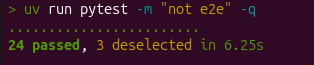
\includegraphics[width=\linewidth]{SS36.png}
		\caption{Fast tests: 24 passed, 3 deselected.}
	\end{subfigure}\hfill
	\begin{subfigure}[t]{0.45\linewidth}
		\centering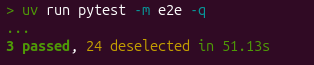
\includegraphics[width=\linewidth]{SS37.png}
		\caption{End-to-end tests: 3 passed, 24 deselected.}
	\end{subfigure}
	\caption{Test evidence for Tasks 3 and 4.}
	\label{fig:tests}
\end{figure}

\section{Results on Our Capture}\label{sec:realtime-results}

Of 569 flows, 22 were dropped (protocol 0) and 547 were classified, all of them as BENIGN: the detector raised 0 DDoS alerts (Table~\ref{tab:t5rt}, Figure~\ref{fig:ss38}). No infinite or NaN cells had to be replaced. Our traffic is benign by construction, so every flow is correctly classified and there is no false positive.

\begin{table}[ht]
	\centering\small
	% AUTO-GENERATED by scripts/make_report_tables.py from outputs/realtime/run_log.txt, outputs/realtime/predictions.csv -- do not edit
\begin{tabular}{lr}
\toprule
Quantity & Value \\
\midrule
Flows read & 569 \\
Protocol-0 flows dropped & 22 \\
inf/NaN cells replaced & 0 \\
Flows classified & 547 \\
Classified BENIGN & 547 \\
DDoS alerts & 0 \\
Alert rate & 0.00\,\% \\
Latency per flow, mean (ms) & 13.537 \\
Latency per flow, median (ms) & 12.840 \\
\bottomrule
\end{tabular}

	\caption{Real-time run on \texttt{task2\_lab2.pcap\_Flow.csv}.}
	\label{tab:t5rt}
\end{table}

\ssfig[0.6\linewidth]{SS38}{Summary of the real-time detector: 569 flows read, 22 Protocol-0 rows dropped, 547 classified, 0 DDoS alerts, mean latency 13.537\,ms per flow.}{fig:ss38}

\section{Latency and Scope}\label{sec:latency}

Classifying one flow at a time takes 13.537\,ms on average (median 12.840\,ms) in our recorded run. This is per-call pandas and scikit-learn overhead: batched, the same model needs 0.695\,ms per 1,000 flows (Table~\ref{tab:t4binary}). In practice, the detection delay is dominated by CICFlowMeter, which emits a flow only when it ends (FIN or RST) or times out (5\,s activity, 120\,s flow timeout). ``Real time'' here means streaming the flows of a recorded capture through the detector one by one; we do not capture packets live.

\paragraph{Limitations of this check.} Our capture contains only benign traffic, so we can measure the false-positive behavior on our network but not the detection rate: whether the model would flag a real DDoS attack in our flows remains untested. In addition, there is domain shift. The training data was produced by an older CICFlowMeter version on the 2017 testbed, whereas our flows come from CICFlowMeter V4 on a different network with a different application mix (for example QUIC and Steam traffic). A model that relies on testbed-specific shortcut features, such as the destination port, may behave differently on other traffic, in either direction.

\FloatBarrier

	% !TeX encoding = UTF-8
\chapter{Discussion and Conclusion}\label{chap:discussion}

\paragraph{Shortcut features and domain shift.} The near-perfect benchmark scores (DDoS F1 0.9996) may partly rest on a shortcut. \texttt{Destination Port} ranks second among the selected features, and virtually all DDoS flows target port 80, so the model may have learned the port rather than the attack behavior (Section~\ref{sec:t3-interp}). The test split comes from the same capture as the training data, so it cannot reveal such a shortcut. The CICFlowMeter version, the hosts and the application mix also differ between the 2017 testbed and our network (Section~\ref{sec:latency}). The 0 alerts on our capture show only that this particular benign traffic is not mistaken for DDoS. The data itself also has quality problems, such as the duplicated column, infinite values, 2,633 duplicate rows and several TCP flag columns that are identical or constant. They match issues reported in the literature~\cite{engelen2021troubleshooting}, and each of them needed its own cleaning step in Chapter~\ref{chap:task3_preprocessing}.

\paragraph{Class balance.} Because the classes are close to balanced, class weighting has almost no effect: the balanced and default Decision Trees are identical on the test split, and the balanced Logistic Regression removes only 34 of about 2,000 false alarms.

\paragraph{Limitations.} We use a single train/test split without cross-validation. The tree is unpruned. We ran no ablation without \texttt{Destination Port}, so we cannot quantify the shortcut. Dropping rows with infinite values removes 34 flows, including 2 DDoS flows, and min-max scaling is sensitive to outliers. Finally, the real-time part replays recorded flows and is not live capture.

\paragraph{Possible improvements (not implemented).} Pruning the tree (\texttt{max\_depth}, \texttt{min\_samples\_leaf}), dropping the testbed-specific features (such as \texttt{Destination Port}), evaluating on a second attack capture from another network, and adding benign traffic from the deployment network to the training data would make the conclusions more reliable.

\paragraph{Conclusion.} We turned the Friday DDoS file of CIC-IDS2017 into a clean set of 223,082 flows with 59 features, selected the 20 best features, and trained Logistic Regression and Decision Tree classifiers for BENIGN vs.\ DDoS. The Decision Tree outperforms Logistic Regression and makes only 32 errors on 66,925 test flows. On our own benign traffic, it raised no false alarm, but because our capture has no attack and the data may allow shortcuts, its benchmark score does not by itself show how well it would detect DDoS attacks in our network.

	
	% -- Appendix (optional, left out for now: the template's Code/Math/Dataset chapters are empty)
	% \begin{appendices}
		%     % !TeX spellcheck = en_US
% !TeX encoding = UTF-8
\chapter{Code}

\chapter{Math}

\chapter{Dataset}
		% \end{appendices}
	% \newpage
	
	
	%%%%%%%%%%%%%%%%%%%%%%%%%%%%%%%%%%%%%%%%%%%%%%%%%%%%%%%%%%%%%%%%%%%%%%%%%%%%%%%%%%%%%%%%%
	\backmatter
	
	% -- Bibliography
	\printbibliography
	
	% -- Eidesstattliche Erklärung (= Affadavit)
	\clearpage
	% !TeX spellcheck = de_DE
% !TeX encoding = UTF-8
\begin{german}
\chapter{Eidesstattliche Erklärung}

	Hiermit versichere ich, dass ich diese \thesisType{} selbstständig und ohne Benutzung anderer als der angegebenen Quellen und Hilfsmittel angefertigt habe und alle Ausführungen, die wörtlich oder sinngemäß übernommen wurden, als solche gekennzeichnet sind, sowie, dass ich die \thesisType{} in gleicher oder ähnlicher Form noch keiner anderen Prüfungsbehörde vorgelegt habe.

	\vspace{3cm}

	Passau, \thedate

	\vspace{2cm}

	\parbox{7cm}{\hrule \strut Justlyn Kaniyanthara Johnson}
	\hfill
	\parbox{7cm}{\hrule \strut Aayush Kapoor}
\end{german}

	
	
\end{document}
